% https://davidstutz.de/illustrating-convolutional-neural-networks-in-latex-with-tikz/
%\documentclass[twoside,11pt,a4paper]{standalone}
\documentclass{standalone}
 
\usepackage[utf8]{inputenc}
\usepackage{amsmath, amssymb, latexsym}
\usepackage{sidecap}
 
\usepackage{tikz}
\usetikzlibrary{decorations.pathreplacing}
 
\begin{document}
 

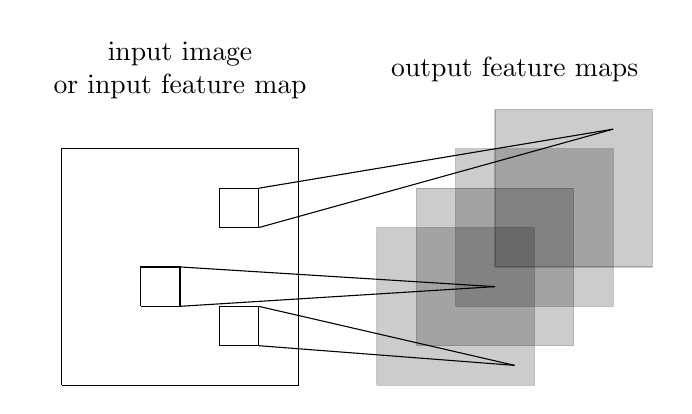
\begin{tikzpicture}
	\node at (1.5,4){\begin{tabular}{c}input image\\or input feature map\end{tabular}};

	\draw (0,0) -- (3,0) -- (3,3) -- (0,3) -- (0,0);
	
	\draw (2,2) -- (2.5,2) -- (2.5,2.5) -- (2,2.5) -- (2,2);
	\draw (2,0.5) -- (2.5,0.5) -- (2.5,1) -- (2,1) -- (2,0.5);
	\draw (1,1) -- (1.5,1) -- (1.5,1.5) -- (1,1.5) -- (1,1);
	
	\draw (2.5,2) -- (7,3.25);
	\draw (2.5,2.5) -- (7,3.25);

	\draw (2.5,1) -- (5.75,0.25);
	\draw (2.5,0.5) -- (5.75,0.25);
	
	\draw (1.5,1.5) -- (5.5,1.25);
	\draw (1.5,1) -- (5.5,1.25);
	
	\node at (5.75,4){\begin{tabular}{c}output feature maps\end{tabular}};
	
	\draw[fill=black,opacity=0.2,draw=black] (5.5,1.5) -- (7.5,1.5) -- (7.5,3.5) -- (5.5,3.5) -- (5.5,1.5);
	\draw[fill=black,opacity=0.2,draw=black] (5,1) -- (7,1) -- (7,3) -- (5,3) -- (5,1);
	\draw[fill=black,opacity=0.2,draw=black] (4.5,0.5) -- (6.5,0.5) -- (6.5,2.5) -- (4.5,2.5) -- (4.5,0.5);
	\draw[fill=black,opacity=0.2,draw=black] (4,0) -- (6,0) -- (6,2) -- (4,2) -- (4,0);
\end{tikzpicture}

\end{document}

